\section{Zuständigkeiten (TiK)}
\label{section_zustaendigkeiten}
<<<<<<< HEAD
In diesem Kapitel wird auf die Zuständigkeiten in Bezug auf die Informationsbereitstellung an der Hochschule Emden/Leer näher eingegangen. Es wird dargestellt, welche Bereiche bereits zentral an der Informationsbereitstellung beteiligt sind. Ebenso wird auf die Besonderheiten einzelner Fachbereiche, zentraler Einrichtungen und dem Präsidium detaillierter eingegangen (siehe Abbildung \ref{fig_organigramm_HS}). 
=======
In diesem Kapitel wird auf die Zuständigkeiten im Bezug auf die Informationsbereitstellung an der Hochschule Emden/Leer näher eingegangen. Es wird dargestellt, welche Bereiche bereits zentral an der Informationsbereitstellung beteiligt sind. Ebenso wird auf die Besonderheiten einzelner Fachbereiche, zentraler Einrichtungen und dem Präsidium detaillierter eingegangen (siehe Abbildung \ref{fig_organigramm_HS}). 
>>>>>>> master

\begin{figure}[h!]
	\centering
	\includegraphics[width=14cm]{kapitel/gruppe2/bilder/organigramm_HS}
	\caption{Organigramm der Hochschule Emden/Leer}
	\label{fig_organigramm_HS}
\end{figure}

Nachfolgend wird ein Überblick über die IT-Systeme gegeben, welche sowohl von Mitarbeitern als auch Studierenden verwendet werden (siehe Abbildung  \ref{fig_zentrale_systeme}). Bei allen zentralen Systemen ist bereits eine Authentifizierung über Single Sign On (SSO) gegeben (siehe Kapitel 3.2.1.1).

\begin{figure}[h!]
	\centering
<<<<<<< HEAD
	\includegraphics[width=14cm]{kapitel/gruppe2/bilder/zentrale-Systeme}
=======
	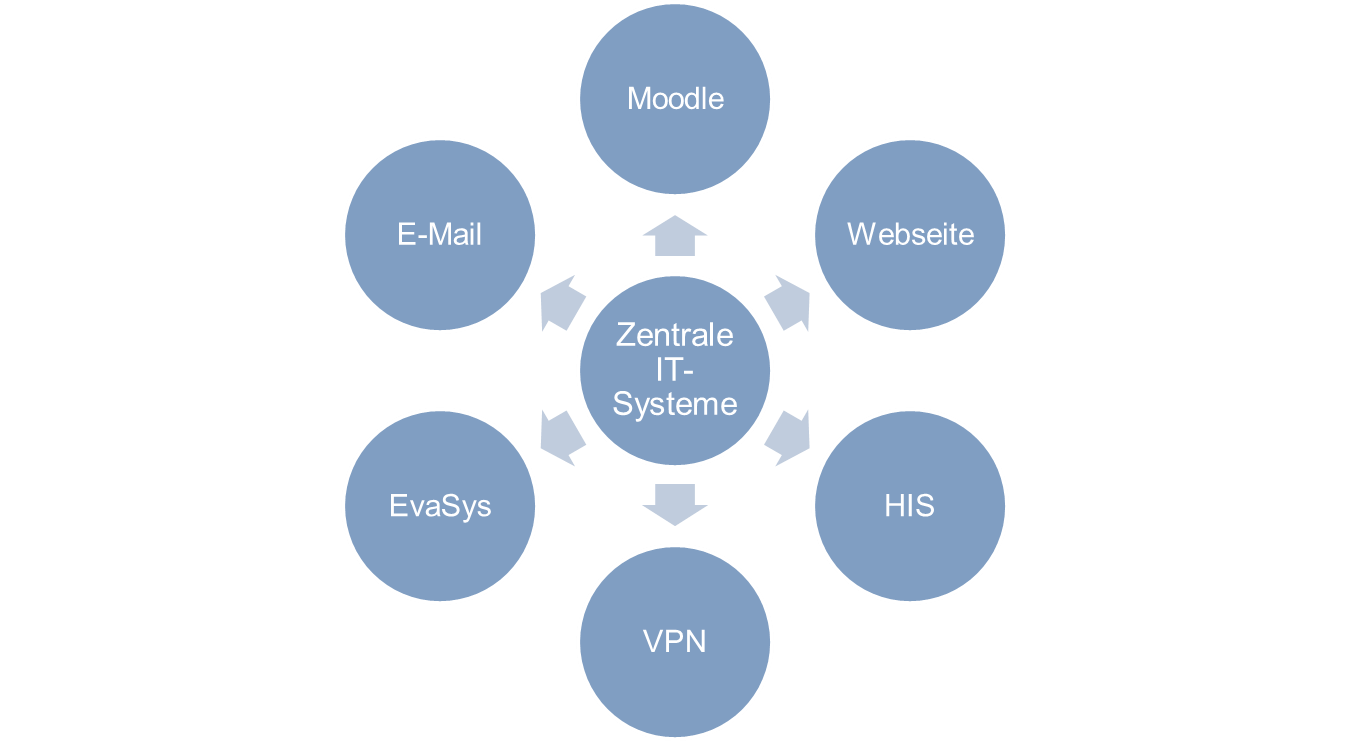
\includegraphics[width=14cm]{kapitel/gruppe2/bilder/zentrale_systeme}
>>>>>>> master
	\caption{Zentrale Systeme für Mitarbeiter und Studenten}
	\label{fig_zentrale_systeme}
\end{figure}


\subsection{Fachbereiche}
Die einzelnen Fachbereiche sind unter anderem durch die Mitgliedschaft in Arbeitsgruppen in den Informationsbeschaffungsprozess involviert.

<<<<<<< HEAD
Alle Fachbereiche verfügen über die Berechtigung, relevante Informationen im Infosys darzustellen. Beim InfoSys handelt es sich um eine zentrale Plattform zur Darstellung von organisatorischen Informationen. Diese können direkt online auf der öffentlichen Webseite der Hochschule Emden/Leer eingesehen werden oder in den Eingangsbereichen der jeweiligen Fachbereiche vor Ort über entsprechende Monitore. Es werden, nach Fachbereich sortiert, die wichtigsten Neuigkeiten als Newsticker dargestellt und der Zugriff auf alle Vorlesungspläne der Fachbereiche ist gegeben, um so zügig auf organisatorische Inhalte zugreifen zu können (siehe Abbildung \ref{fig_InfoSys}). Aufbauend auf dem InfoSys wird eine selbst entwickelte Android App zur Verfügung gestellt.

%\begin{figure}[h!]
%	\centering
%	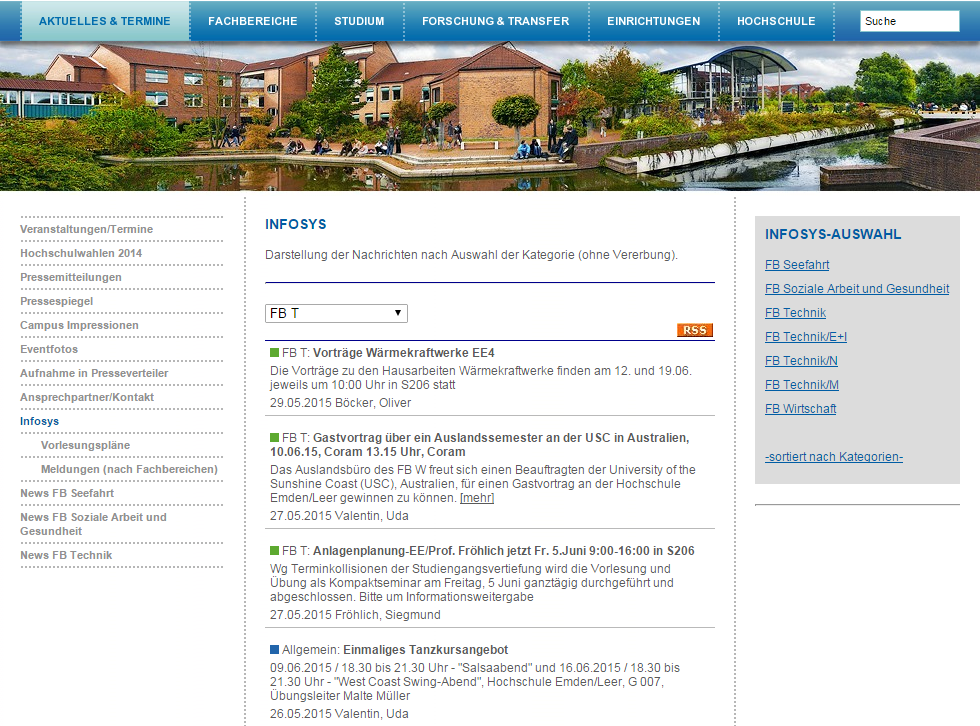
\includegraphics[width=14cm]{kapitel/gruppe2/bilder/InfoSys}
%	\caption{Exemplarischer Screenshot des INFOSYS des Fachbereiches Technik}
%	\label{fig_InfoSys}
%\end{figure}
\missingfigure{Abbildung InfoSys}
=======
Alle Fachbereiche verfügen über die Berechtigung relevante Informationen im Infosys darzustellen. Beim InfoSys handelt es sich um eine zentrale Plattform zur Darstellung von organisatorischen Informationen. Diese können direkt online auf der öffentlichen Webseite der Hochschule Emden/Leer eingesehen werden oder in den Eingangsbereichen der jeweiligen Fachbereiche vor Ort über entsprechende Monitore. Es werden, nach Fachbereich sortiert, die wichtigsten Neuigkeiten als Newsticker dargestellt und der Zugriff auf alle Vorlesungspläne der Fachbereiche ist gegeben um so zügig auf organisatorische Inhalte zugreifen zu können (siehe Abbildung \ref{fig_InfoSys}). Aufbauend auf dem InfoSys wird eine selbst entwickelte Android App zur Verfügung gestellt.

\begin{figure}[h!]
	\centering
	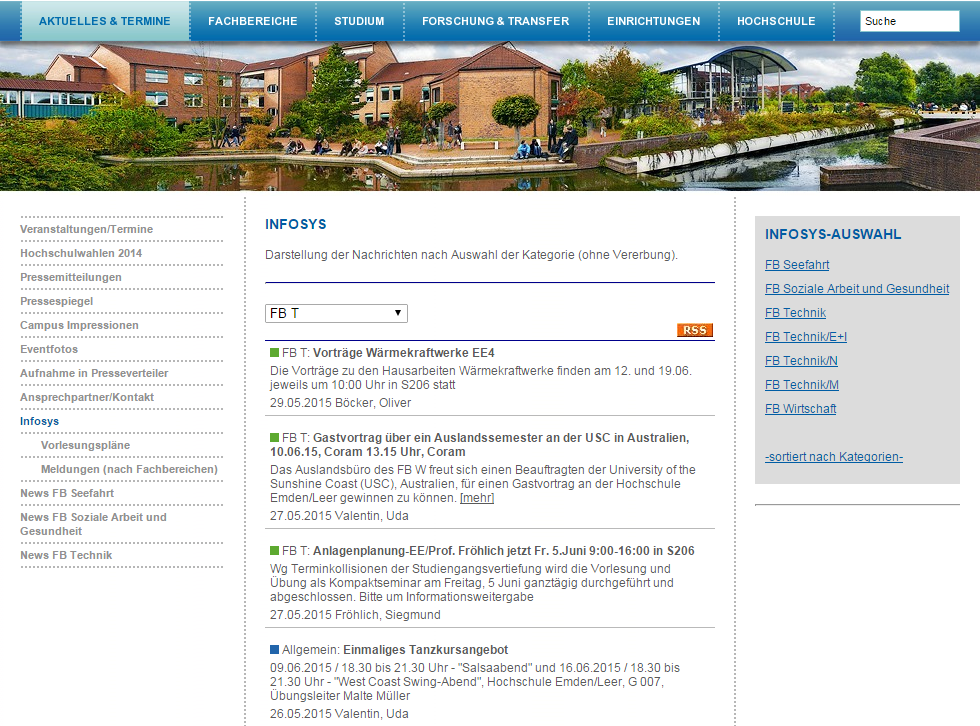
\includegraphics[width=14cm]{kapitel/gruppe2/bilder/InfoSys}
	\caption{Exemplarischer Screenshot des INFOSYS des Fachbereiches Technik}
	\label{fig_InfoSys}
\end{figure}
>>>>>>> master

In den nachfolgenden Kapiteln wird auf die Besonderheiten der einzelnen Fachbereiche eingegangen.

\subsubsection{Seefahrt}
Bei dem Fachbereich Seefahrt handelt es sich um einen relativ kleinen Fachbereich. Seefahrt ist  nur an dem Standort Leer vertreten. Dieser Fachbereich verwendet kein zentrales System zur Vorlesung und Raumplanung, sondern eine Eigenentwicklung.

\subsubsection{Technik}
Eine Besonderheit dieses Fachbereiches ist, dass für den Laborbetrieb ein Netzwerk neben dem zentralen Netzwerk der Hochschule Emden/Leer betrieben wird. Da unter anderem der Bereich „IT-Sicherheit“ ein wichtiger Aspekt in dem Studiengang Informatik ist, kommt es zu besonderen Konstellationen im Bereich der Forschung. Dieser Bereich verwaltet sein Netz selbst und ist somit autark vom allgemeinen Hochschulrechennetz. Es besteht jedoch eine enge Zusammenarbeit zwischen dem Bereich Technik (im speziellen E+I) und dem Rechenzentrum, so dass unter anderem gegenseitige Zugriffsrechte bestehen. 

\subsection{Präsidium}
<<<<<<< HEAD
\label{subsection_prasidium}
Das Präsidium, insbesondere mit dem Bereich zentrale Verwaltung, ist über  Arbeitsgruppen in den Informationsbeschaffungsprozess involviert. Zudem verfügt das Präsidium mit einer Stabsstelle über einen zentralen Bereich im Bezug auf die Repräsentation von Informationen.  Das Präsidialbüro ist unter anderem für den Bereich Hochschulmarketing zuständig. Auch ist in der Stabstelle des Präsidialbüros die Presse- und Öffentlichkeitsarbeit angesiedelt.
=======
\label{subsection_zustaendigkeiten_praesidium}
Das Präsidium insbesondere mit dem Bereich zentrale Verwaltung ist über  Arbeitsgruppen in den Informationsbeschaffungsprozess involviert. Zudem verfügt das Präsidium mit einer Stabsstelle über einen zentralen Bereich im Bezug auf die Repräsentation von Informationen.  Das Präsidialbüro ist unter anderem für den Bereich Hochschulmarketing zuständig. Auch ist in der Stabstelle des Präsidialbüros die Presse- und Öffentlichkeitsarbeit angesiedelt.
>>>>>>> master

\subsection{Zentrale Verwaltung}
Die zentrale Verwaltung verwendet im Bereich Personalverwaltung und Finanzen ausschließlich „SAP“ als Buchhaltungssystem. Zur Organisation von Lehr- und Vorlesungsplanung wird das System UNTIS Plus verwendet. Ebenso wird für die Urlaubsplanung, Zeiterfassung und das Gebäudeschließsystem ein eigenständiges Programm verwendet.Speziell für die Aufbereitung von Kennzahlen und Zahlen wird eine Eigenentwicklung als Business Intelligence System verwendet. 

\subsubsection{Studentenverwaltung}
\subsubsection{Mitarbeiterverwaltung}
\subsubsection{Rechenzentrum}
Das Hochschulrechenzentrum der Hochschule Emden/Leer ist stark in die Administration und Pflege der bestehenden Systeme zur Informationsbereitstellung involviert. Neben der Administration von bestehenden Systemen obliegt dem Hochschulrechenzentrum ebenfalls der Endkundensupport.

\subsection{Arbeitsgruppen zum Informationsaustausch und zur Informationsbereitstellung}
\label{subsection_arbeitsgruppen_informationsaustausch}
Die Zuständigkeiten an der Hochschule, in Bezug auf Informationssammlung, Beschaffung und Aufbereitung von Informationen, ist bereits durch Arbeitsgruppen in wichtigen Bereichen geregelt. Durch das Interview mit dem Leiter des Hochschulrechenzentrums der Hochschule Emden/Leer konnte ein Einblick in die bestehenden Gremien geschaffen werden. Diese treffen sich regelmäßig zum Informations-, Wissens- und Erfahrungsaustausch.

Es existieren drei Arbeitsgruppen, welche für die Informationsverteilung in den jeweiligen Bereichen relevant sind:

\begin{itemize}
	\item Zahlen, Daten und Fakten (ZDF)
	\item WEB
	\item Moodle
\end{itemize}

\subsubsection{Zahlen, Daten und Fakten (ZDF)}
<<<<<<< HEAD
ZDF setzt sich zusammen aus den Verwaltungsabteilungen Finanzen, Personal, Presse und Rechenzentrum. Dieses Gremium ist zuständig für die Erstellung und Aufbereitung von Kennzahlen. Dies können zum Beispiel aktuelle Kennzahlen zu eingeschriebenen Studierenden pro Studiengang sein.  ZDF ist für einen Unterbereich der offiziellen Webseite der Hochschule Emden/Leer zuständig. Die Kennzahlen und Zahlen werden gruppenbasiert erstellt. Je nach Berechtigung werden Kennzahlen in unterschiedlichen Detailgraden dargestellt. So erhalten Dekane mehr Informationen als Mitarbeiter. Öffentlich zugänglich sind nur generische Kennzahlen. 
=======
ZDF setzt sich zusammen aus den Verwaltungsabteilungen Finanzen, Personal, Presse und Rechenzentrum. Dieses Gremium ist zuständig für die Erstellung und Aufbereitung von Kennzahlen. Dies können zum Beispiel aktuelle Kennzahlen zu eingeschriebenen Studierenden pro Studiengang sein.  ZDF ist für einen Unterbereich der offiziellen Webseite der Hochschule Emden/Leer zuständig. Die Kennzahlen und Zahlen werden gruppenbasiert erstellt. Je nach Berechtigung werden Kennzahlen in unterschiedlichen Detailgraden dargestellt. So erhalten Dekane mehr Informationen als Mitarbeiter und öffentlich zugänglich sind nur generische Kennzahlen. 
>>>>>>> master

\subsubsection{WEB}
Es existiert eine Arbeitsgruppe, welche für die Gestaltung und den Inhalt der öffentlichen Webseite der Hochschule Emden/Leer verantwortlich ist. In dieser Arbeitsgruppe sind aus jedem Fachbereich Repräsentanten mit einbezogen. Die Leitung des Web-Teams obliegt dem Präsidialbüro.\footnote{\url{http://www.hs-emden-leer.de/fileadmin/user_upload/Einrichtungen/Praesidialbuero/Organigramm_Praesidialbuero_Juli2013_01.pdf}}

\subsubsection{Moodle}
In der Arbeitsgruppe „Moodle“ sind sowohl Repräsentanten aus jedem Fachbereich involviert sowie auch Repräsentanten aus der Verwaltungsebene. Da das Moodle E-learning System mittlerweile als ein zentrales Moodle für alle Bereiche eingeführt wurde, haben die Mitglieder aus den Fachbereichen unter anderem das Recht Kurse im Moodle freischalten zu können. Auf die E-Learning Plattform „Moodle“ wird detaillierter im Kapitel 2.4.3 eingegangen.
